%% Sets aspect ratio to 16:10, and frame size to 160mm by 100mm
% Please, do not use old-school 4:3 ratio anymore:)
\documentclass[aspectratio=1610]{beamer}
% všechny soubory jsou v utf-8
\usepackage{ucs}% pro kódování UTF-8
\PrerenderUnicode{ěščřžýáíéĚŠČŘŽÝÁÍÉďťňĎŤŇůúÚóÓ} % předkreslení diakritiky, možno přidat/ubrat znaky podle potřeby	

%% Select your favorite language
%\usepackage[english]{babel} % Multilingual support for LaTeX
\usepackage[czech]{babel}
\usepackage[IL2]{fontenc}% csr fonty (pokud jsou nainstalovány česká postscriptová mísma)

\usepackage[utf8]{inputenc} % Accept different input encodings
\usepackage{graphicx} % Enhanced support for graphics
\usepackage{listings} % Typeset source code listings using LaTeX
\usepackage{color} % Colour control for LaTeX documents

%% Copy your favorite logo from "vut_logo_archive/" to root folder 
% and rename file to "logo.png"

%% Select color theme
\usepackage[FSI]{themevut}

% ----------------------------------------------------------------------
% TITLE PAGE
% ----------------------------------------------------------------------

% The short title appears at the bottom of every slide, the full title
% is only on the title page.
\title[Sémantická segmentace obrazu pomocí CNN]
{Sémantická segmentace obrazu pomocí konvolučních neuronových sítí}

% Type of project, i.e. Bachelor, Master, PhD, etc.
\subtitle
{Diplomová práce}

% Your name
\author[Bc. Filip Špila]
{Bc. Filip Špila \\
	\texttt{filipspila@gmail.com}}

% Your institution
\institute
{Ústav mechaniky těles, mechatroniky a biomechaniky \\
	Vysoké učení technické v Brně
}

% Date, can be changed to a custom date
\date{\today}

% Logo on title page
\titlegraphic{
\includegraphics[height=.1\textheight]{logo4.png}}

\begin{document}
	
	% ----------------------------------------------------------------------
	% PRESENTATION SLIDES
	% ----------------------------------------------------------------------
	
	\begin{frame}
	% Print the title page as the first slide
	\titlepage
\end{frame}

% ----------------------------------------------------------------------
% https://cs.overleaf.com/learn/latex/Lists

\begin{frame}{Cíle práce}
\begin{enumerate}
	\item Nastudování problematiky segmentace obrazu pomocí konvolučních neuronových sítí
	\item Výběr perspektivní architektury sítě spolu s její implementací
	\item Vytvoření vlastní trénovací množiny obrázků
	\item Vytvoření segmentovaného obrazu
	\item Vyhodnocení úspěšnosti segmentace
\end{enumerate}	
	
\begin{center}
	\begin{figure}
		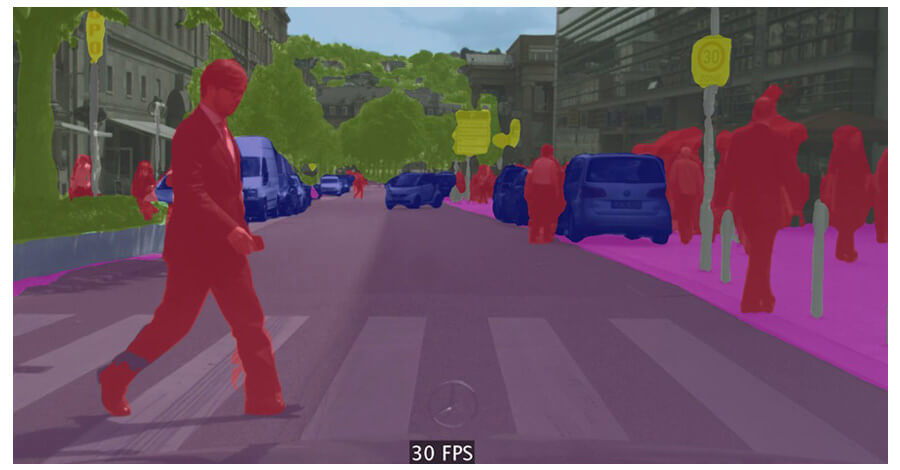
\includegraphics[width=5.5cm]{semseg.jpg}	
		\caption{Sémantická segmentace}		
	\end{figure}	
\end{center}
\end{frame}

% ----------------------------------------------------------------------

\begin{frame}{Sémantická segmentace}

\textbf{Cíle sémantické segmentace}
	\begin{itemize}
	\item Přiřadit každému pixelu v obrázku právě jednu třídu objektu (auto, člověk, zvíře, ...)
	% Narozdil od klasifikace obrazu jako celku
	\item Provádět segmentaci co nejpřesněji
	% Tedy s presnym vykreslenim hranice kazdeho objektu
	\item Zajistit, aby algoritmus uměl generalizovat
	% Tedy aby spravne klasifikoval objekty bez ohledu na svetelne podminky, ruzne nedokonalosti atp.	
	\end{itemize}
		
	\begin{center}
		\begin{figure}
			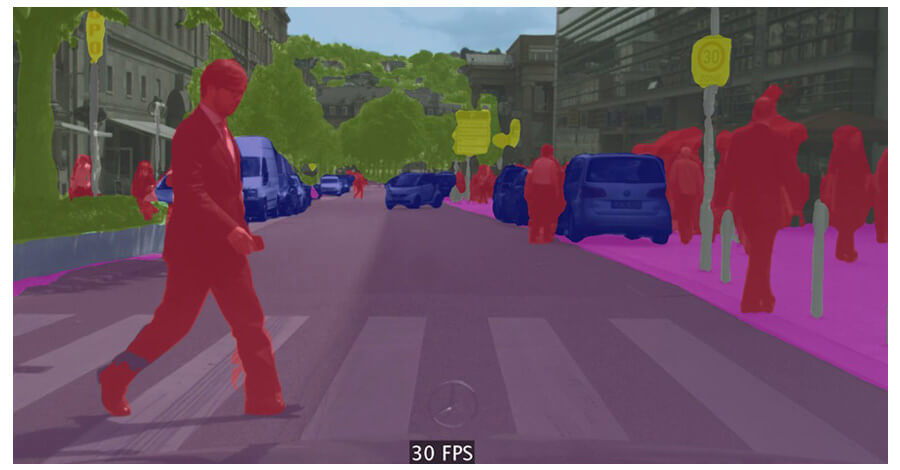
\includegraphics[width=6.5cm]{semseg.jpg}	
			\caption{Sémantická segmentace}		
		\end{figure}	
	\end{center}
\end{frame}

% ----------------------------------------------------------------------
% https://en.wikibooks.org/wiki/LaTeX/Floats,_Figures_and_Captions
\begin{frame}{Figure}
\begin{center}
\begin{figure}

\includegraphics[width=0.3\textwidth]{logo4.png}
\caption{Your caption}
\end{figure}
\end{center}
\end{frame}

% ----------------------------------------------------------------------
% https://en.wikibooks.org/wiki/LaTeX/Tables
\begin{frame}{Table}
\begin{center}
\begin{table}
\caption{Your caption}
\begin{tabular}{l | c | c | c | r}
\textbf{Function name} & \textbf{Duration} & \textbf{Complexity} & \textbf{Length} & \textbf{Score}\\
\hline \hline
Algo 1 & 0.0159 & 0.50 & 125 & 78 \\
Algo 2 & 0.0453 & 0.65 & 854 & 88 \\
Algo 3 & 0.8642 & 0.77 &  84 & 95 \\
Algo 4 & 0.0020 & 0.24 & 638 & 76 \\
\end{tabular}
\end{table}
\end{center}
\end{frame}

% ----------------------------------------------------------------------
% https://en.wikibooks.org/wiki/LaTeX/Mathematics
\begin{frame}{Equations}
Pythagorean theorem can be written in one short equation as: $a^2 + b^2 = c^2$ where $c$ is the longest side of the triangle, $a$ and $b$ are the other two sides.

\vfill % Rubber length which can stretch or shrink vertically

Other useful equations (thank you \textit{John Napier}):
\begin{equation}
\log_b (x\cdot y) = \log_b (x) + \log_b (y)
\end{equation}
\begin{equation}
\log_b \left( \frac{x}{y} \right) = \log_b (x) - \log_b (y)
\end{equation}
\begin{equation}
\log_b (x^p) = p\cdot \log_b (x)
\end{equation}
\begin{eqnarray}
\log_b(x) = y & \text{exactly if} & b^y = x\
\end{eqnarray}
\end{frame}

% ----------------------------------------------------------------------
% https://cs.overleaf.com/learn/latex/Code_listing
\begin{frame}[fragile]{Code listings}
% Need to use the "fragile" option when verbatim is used in the slide

\begin{lstlisting}[language=C,title={Sample code in C}]
void setup(void) {
uart_init(UART_BAUD_SELECT(UART_BAUD_RATE, F_CPU));  // UART mode 8N1
esp8266_init();  // Initialize ESP8266 Wi-Fi module
}
\end{lstlisting}
\vfill

\begin{lstlisting}[language=vhdl,title={Sample code in VHDL}]
---------------------------------------------------------------
-- Entity declaration for hexadecimal to seven-segment decoder
---------------------------------------------------------------
entity hex_to_7seg is
port (hex_i: in  std_logic_vector(4-1 downto 0);
seg_o: out std_logic_vector(7-1 downto 0));
end entity hex_to_7seg;
\end{lstlisting}

\begin{lstlisting}[language=Matlab,title={Sample code in Matlab}]
x = 0:0.05:5;
y = sin(x.^2);
figure
plot(x,y)  % The plot function creates simple line plots of x and y values
\end{lstlisting}
\end{frame}

% ----------------------------------------------------------------------
% Remind the main results at the end of your presentation
\begin{frame}{Achieved results}
\begin{itemize}
\item Lorem ipsum dolor sit amet, consectetuer adipiscing elit.
\item Etiam sapien elit, consequat eget, tristique non, venenatis quis, ante.
\item Aliquam erat volutpat.
\item Integer lacinia.
\item Cras pede libero, dapibus nec, pretium sit amet, tempor quis.
\end{itemize}
\end{frame}

% ----------------------------------------------------------------------
% It is a common practice you already have reviewer(s) comments/questions before your presentation. Sometimes, it is useful to prepare extra slides to answer those questions.
\begin{frame}{Reviewer's questions}
\begin{columns}
\column{0.45\textwidth}
\begin{exampleblock}{Question 1}
Lorem ipsum dolor sit amet, consectetur adipiscing elit. Integer lectus nisl, ultricies in feugiat rutrum, porttitor sit amet augue. Aliquam ut tortor mauris. Sed volutpat ante purus, quis accumsan dolor.
\end{exampleblock}

\column{0.45\textwidth}
\begin{block}{Answer 1}
Lorem ipsum dolor sit amet, consectetur adipiscing elit. Integer lectus nisl, ultricies in feugiat rutrum, porttitor sit amet augue. Aliquam ut tortor mauris. Sed volutpat ante purus, quis accumsan dolor.
\end{block}
\end{columns}
\end{frame}

% ----------------------------------------------------------------------

\end{document}
